\documentclass[11pt,a4paper]{article}
\usepackage[T1]{fontenc}
\usepackage{tgpagella,tgheros}
\usepackage[margin=22mm,top=21mm,bottom=22mm,headsep=11pt,footskip=22pt]{geometry}
\usepackage{amsmath,graphicx,booktabs,tabularx,array,longtable,xcolor,caption,fancyhdr}
\usepackage[numbers,sort&compress]{natbib}
\usepackage[hyphens]{url}
\usepackage[hidelinks]{hyperref}

\definecolor{teal}{HTML}{10655C}
\definecolor{ink}{HTML}{243235}
\definecolor{rulegray}{HTML}{8FA8A3}
\definecolor{paper}{HTML}{F1F7F5}
\color{ink}
\hypersetup{pdftitle={HAM10000 Skin Lesion Classification},pdfauthor={Team 16, IIITDM Kancheepuram}}
\setlength{\parindent}{0pt}
\setlength{\parskip}{5pt plus 1pt}
\setlength{\headheight}{15pt}
\setlength{\emergencystretch}{2em}
\setlength{\tabcolsep}{5pt}
\renewcommand{\arraystretch}{1.19}
\raggedbottom
\widowpenalty=10000
\clubpenalty=10000
\newcolumntype{Y}{>{\raggedright\arraybackslash}X}
\newcolumntype{L}[1]{>{\raggedright\arraybackslash}p{#1}}
\makeatletter
\renewcommand\section{\@startsection{section}{1}{\z@}%
  {-2.4ex plus -.5ex minus -.2ex}{.8ex plus .2ex}{\sffamily\Large\bfseries\color{teal}}}
\renewcommand\subsection{\@startsection{subsection}{2}{\z@}%
  {-1.7ex plus -.4ex minus -.2ex}{.4ex plus .1ex}{\sffamily\normalsize\bfseries}}
\makeatother
\captionsetup{font=small,labelfont={sf,bf},labelsep=period,justification=raggedright,
  singlelinecheck=false,hypcap=false,skip=5pt}
\pagestyle{fancy}
\fancyhf{}
\fancyhead[L]{\sffamily\scriptsize\bfseries TEAM 16}
\fancyhead[R]{\sffamily\scriptsize HAM10000 SKIN LESION CLASSIFICATION}
\fancyfoot[C]{\sffamily\footnotesize\thepage}
\renewcommand{\headrulewidth}{.35pt}

\newcommand{\reportfigure}[4]{%
  \par\medskip
  \begin{minipage}{\linewidth}
    \centering
    \includegraphics[width=#1\linewidth,keepaspectratio]{figures/#2}
    \captionof{figure}{#3}\label{#4}
  \end{minipage}\par\smallskip}
\newcommand{\screenframe}[1]{%
  {\setlength{\fboxsep}{0pt}\color{rulegray}\fcolorbox{rulegray}{paper}{%
    \rule{0pt}{#1}\rule{\dimexpr\linewidth-2\fboxrule\relax}{0pt}}}}
\newcommand{\screen}[3][]{%
  \includegraphics[width=\linewidth,height=#2,keepaspectratio,#1]{figures/#3}}

\begin{document}

\hypersetup{pageanchor=false}
\begin{titlepage}
\thispagestyle{empty}
\vspace*{28mm}
\begin{center}
{\sffamily\bfseries\small\color{teal} IIITDM KANCHEEPURAM\par}
\vspace{11mm}
{\color{teal}\rule{.87\linewidth}{.8pt}\par}
\vspace{9mm}
{\sffamily\bfseries\fontsize{27}{32}\selectfont Skin Lesion Classification\\[2pt] on HAM10000\par}
\vspace{4mm}
{\large Lesion-grouped evaluation under class imbalance\par}
\vspace{9mm}
{\color{teal}\rule{.87\linewidth}{.45pt}\par}
\vspace{12mm}
{\sffamily\bfseries Team 16\par}
\vspace{4mm}
{\renewcommand{\arraystretch}{1.5}
\begin{tabular}{@{}l@{\hspace{15mm}}l@{}}
N. Deepak & CS24B1044\\
V. Sai Nikhil & CS24B1053\\
S. Sai Lohith & CS24B1087\\
D. Revanth Reddy & CS24B1080
\end{tabular}\par}
\vspace{13mm}
{\sffamily\bfseries Introduction to Data Science for Engineers\par}
\vspace{2mm}
Dr. Jagadeesh Kakarla\par
\vspace{3mm}
Live demo: \href{https://skin-lesion-classification-umber.vercel.app/}{https://skin-lesion-classification-umber.vercel.app/}
\end{center}
\end{titlepage}
\hypersetup{pageanchor=true}

\section{Abstract}
We studied how class imbalance affects dermoscopic skin lesion classification on HAM10000. The dataset contains 10,015 images across seven classes, with many more images of melanocytic nevi than of the rarest lesions. We split the data by lesion and removed near-duplicate images from training. We compared four baselines, four more complex architectures and a final ConvNeXt-Tiny model. Our primary metric was macro-F1, which gives each class equal weight. In the ResNet-50 experiments, per-epoch resampling with near-duplicate removal raised test macro-F1 from 0.6542 to 0.7447 relative to plain training. The selected ConvNeXt-Tiny checkpoint reached 0.7783 macro-F1, 0.8346 accuracy and 0.8123 balanced accuracy without post-hoc adjustment. A four-seed ResNet-50 ensemble reached 0.7815 macro-F1. We examined errors using a row-normalized confusion matrix, Grad-CAM and selected test examples. The expected calibration error was 0.0725, and the highest confidence band was less accurate than the preceding band. We also built an educational web application that displays predictions, optional heatmaps and a PDF summary. The evaluation concerns the held-out HAM10000 split.

\section{Introduction}
HAM10000 brings together dermoscopic images of common pigmented skin lesions \citep{tschandl2018}. A classifier trained on these images must distinguish conditions that can resemble one another while learning from very different numbers of examples per class. Accuracy gives each image the same weight. On an imbalanced test set, this places much of the aggregate weight on the common categories. We used macro-F1 to give each class an equal place in model comparison.

The unit of observation also matters. The collection can include several photographs of one lesion. An image-level split can place photographs of the same lesion on both sides of the evaluation. We assigned lesion identifiers to disjoint splits and checked for image similarity beyond those identifiers. This setup kept the held-out class distributions intact and let us change the way the training data were sampled.

We asked how much of the performance difference came from training choices within a single architecture and how much appeared when we changed architectures. For the first question, we followed a ResNet-50 through inverse-frequency weighting, resampling, duplicate removal and a fuller optimization recipe. For the second, we compared convolutional models, a transformer and two hybrid designs on the shared split. Several changes occurred together, so we interpret those runs as recipe comparisons.

Our evaluation also considers what the final predictions communicate. We compare precision-sensitive F1 with recall by class, inspect directions of error, and examine the relationship between a model score and correctness. The application exposes the model as a demonstration of this analysis. Its predictions and heatmaps are for educational use.

\clearpage
\section{Survey}
\begingroup
\small
\setlength{\parskip}{4pt}
We grouped the studies by their main contribution. Table~\ref{tab:survey} records the authors' reported measures and the main constraint on comparison with our experiment.

\subsection{Classical Machine Learning}
The feature-based study \citep{surveyFeatures} segments lesions, extracts hand-crafted descriptors, and compares a random forest with a support vector classifier on subsets of ISIC 2019. Balancing the samples raised the random forest's reported five-class accuracy from 73\% to 80\%, while melanoma remained its most difficult class by AUC.

\subsection{Convolutional and Hybrid Networks}
An early-detection CNN study \citep{surveyEarlyCNN} applied resizing and augmentation to HAM10000 and trained a compact network on both the original and balanced sets. Its reported test accuracy increased from 74\% to 83\% after balancing.

The pretrained-network study \citep{surveyPretrained} compared ImageNet backbones while keeping the feature extractors frozen. ConvNeXt-Base led the binary ISIC 2019 experiment with 84.63\% accuracy, on a task that merged the original lesion classes into benign and malignant groups.

Chiu et al. \citep{surveyChiu} tested CNN and transformer backbones on pathology-confirmed hospital images. Their Swin, ViT and EfficientNet-B4 ensemble reached 98.5\% accuracy under repeated holdout, compared with 84.9\% for the best single model.

Gajera et al. \citep{surveyGajera} applied spatial attention followed by channel attention at multiple scales to focus on fine lesion features. With a DenseNet-121 backbone, MTA-Net reached 91.51\% accuracy on HAM10000 and 78.4\% on ISIC 2019.

Saeed et al. \citep{surveySaeed} combined convolutional feature extractors, shifted-window attention and a graph attention block to link visual features before classification. The reported figures for TransXV2S-Net are 95.26\% accuracy and 94.32\% F1, with the evaluation split unspecified.

Mohammed et al. \citep{surveyMohammed} processed clinical and dermoscopic images in separate streams and fused them progressively with attention. Their model added metadata before classification and reported 85.6\% accuracy on the Seven-Point Checklist dataset.

\subsection{Class Imbalance}
Chatterjee et al. \citep{surveyChatterjee} combined pretrained InceptionV3 and Xception with targeted augmentation of rare categories. The study reports a peak accuracy of 98.8\% after balancing and fewer melanoma and basal cell carcinoma errors.

Eva et al. \citep{surveyEva} combined class weighting with selective fine-tuning of EfficientNet-B4 and a custom classification head. They reported 87.95\% macro-F1 and 92.35\% accuracy with test-time augmentation.

Hu et al. \citep{surveyHu} alternated ordinary and balanced batches during training. Their metric-learning term pulled same-class embeddings together and separated different classes, producing 85.92\% accuracy on ISIC 2018 and 83.06\% on ISIC 2019.

Zhang et al. \citep{surveyZhang} used multiple class prototypes to represent variation within each label. Class-dependent feature compression and a balanced contrastive loss yielded 87.66\% F1 on ISIC 2018 and 70.78\% on Derm-SD8 with ResNet-50.

Pak et al. \citep{surveyPak} combined self-supervised and supervised contrastive learning, used a segmentation heatmap to guide attention, and sampled rare classes more often. Their HAM10000 evaluation reported 72.19\% accuracy and 72.96\% weighted F1.

Shah and Khan \citep{surveyShah} used a ResNet-18 encoder and a transformer to combine local and wider spatial information. They downsampled frequent categories, augmented rare ones and reported 97.32\% accuracy on a separate test set at its original class distribution.

\begin{samepage}
\subsection{Explainability and Trust}
The decision-rewriting study \citep{surveyTrust} grouped Grad-CAM maps to find visual shortcuts such as dark borders and rulers. Human rules guided a replacement classifier away from these concepts. The reported melanoma result for dark-corner cases rose from 60.86 to 83.16.

Zuo et al. \citep{surveyZuo} estimated how much to trust predictions from image and metadata branches before combining them. On the Seven-Point Criteria database, uncertainty-based fusion raised average accuracy from 76.2\% to 76.6\%.\par
\end{samepage}

We infer that the published HAM10000 accuracies around 97--99\% are unsuitable for direct comparison with ours because they use different splits and their studies do not state that images were grouped by lesion.
\endgroup
\par\medskip
\begin{minipage}{\linewidth}
\centering
\captionof{table}{Comparison of surveyed skin-lesion classification studies. Results use the measures reported for each study. The final column identifies a constraint on interpretation or comparison.}
\label{tab:survey}
\footnotesize
\setlength{\tabcolsep}{4pt}
\renewcommand{\arraystretch}{1.11}
\begin{tabularx}{\textwidth}{@{}L{.145\textwidth}L{.159\textwidth}L{.18\textwidth}L{.165\textwidth}Y@{}}
\toprule
Paper & Dataset & Method & Reported result & Limitation \\
\midrule
Image features \citep{surveyFeatures} & ISIC 2019 subset & Hand-crafted features, random forest and SVC & 80\% five-class accuracy after balancing & Different label subset \\
Early CNN \citep{surveyEarlyCNN} & HAM10000 & Compact CNN with class balancing & 83\% test accuracy after balancing & Balancing changes the class mix \\
Pretrained CNNs \citep{surveyPretrained} & ISIC 2019 & Frozen backbones with new heads & 84.63\% accuracy & Benign versus malignant task \\
Chiu et al. \citep{surveyChiu} & Hospital dermoscopy & Swin, ViT and EfficientNet-B4 & 98.5\% repeated-holdout accuracy & Single hospital cohort \\
Gajera et al. \citep{surveyGajera} & HAM10000, ISIC 2019 & Multiscale spatial and channel attention & 91.51\%, 78.4\% accuracy & Performance varies across datasets \\
Saeed et al. \citep{surveySaeed} & ISIC 2019, HAM10000 & CNNs, Swin and graph attention & 95.26\% accuracy, 94.32\% F1 & Evaluation split is unspecified \\
Mohammed et al. \citep{surveyMohammed} & Seven-Point Checklist & Progressive image fusion plus metadata & 85.6\% accuracy & Requires paired images and metadata \\
Chatterjee et al. \citep{surveyChatterjee} & HAM10000 & InceptionV3, Xception and rare-class augmentation & 98.8\% peak accuracy & Lesion grouping unreported \\
Eva et al. \citep{surveyEva} & HAM10000 & Weighted EfficientNet-B4 with custom head & 87.95\% macro-F1 & Stratified train--validation split \\
Hu et al. \citep{surveyHu} & ISIC 2018, ISIC 2019 & Balanced batches and metric learning & 85.92\%, 83.06\% accuracy & Accuracy alone does not describe class-level errors \\
Zhang et al. \citep{surveyZhang} & ISIC 2018, Derm-SD8 & Multiple prototypes and contrastive learning & 87.66\%, 70.78\% F1 & Scores vary across datasets \\
Pak et al. \citep{surveyPak} & SLICE-3D, HAM10000 & Contrastive training and heatmap attention & 72.19\% accuracy, 72.96\% weighted F1 & Weighted F1 favors larger classes \\
Shah and Khan \citep{surveyShah} & HAM10000 & ResNet-18 with a transformer & 97.32\% test accuracy & Lesion grouping unreported \\
Decision rewriting \citep{surveyTrust} & ISIC 2019 and 2020 & Grad-CAM concepts and human rules & 60.86 to 83.16 for melanoma with dark corners & Human concept and rule design \\
Zuo et al. \citep{surveyZuo} & Seven-Point Criteria & Uncertainty-guided multimodal fusion & 76.6\% average accuracy & Requires paired inputs and metadata \\
\bottomrule
\end{tabularx}
\end{minipage}

\clearpage
\section{Dataset}
HAM10000 contains 10,015 dermoscopic images from 7,470 lesions \citep{tschandl2018}. We used all seven diagnostic categories. Melanocytic nevi (\texttt{nv}) account for 6,705 images and dermatofibroma (\texttt{df}) for 115. The resulting imbalance ratio is 58.3. The other categories are melanoma (\texttt{mel}), benign keratosis-like lesions (\texttt{bkl}), basal cell carcinoma (\texttt{bcc}), actinic keratoses and intraepithelial carcinoma (\texttt{akiec}), and vascular lesions (\texttt{vasc}). Figure~\ref{fig:counts} shows the counts before partitioning.

\reportfigure{.90}{class_distribution.png}{Full-dataset image counts by diagnostic category.}{fig:counts}

We partitioned by lesion identifier. The training, validation and test partitions contained 7,991, 1,008 and 1,016 images, respectively. We checked that the partitions shared no lesion identifiers. They retained their native class frequencies, leaving a sparse set of examples for several diagnoses.

For the deduplicated recipes, we used difference hashing (\textit{dHash}) to flag visually similar images. The removal threshold was a Hamming distance of 12 or less. We removed 41 training images implicated in near-duplicate pairs. When a training image matched a held-out image, we removed the training image. For matches within training, we kept one of the pair where both were still present. We kept the validation and test cohorts fixed. The audit flagged five validation-to-test pairs, which remain a limitation of evaluation based on lesion identifiers and image hashes.

\reportfigure{.96}{split_and_leakage.png}{Lesion-grouped partition and training-image removal. The hash audit left 7,950 training images.}{fig:split}

\clearpage
\section{Method}
\subsection{Evaluation Protocol}
We used the same lesion-grouped partitions for the project comparisons. Accuracy is the fraction of correctly classified test images. Balanced accuracy averages recall across classes. Macro-F1 first computes F1 for each class from its precision and recall, then averages those class scores with equal weight. Macro-F1 was our primary metric. We chose the main checkpoint using validation macro-F1 and evaluated it on the fixed test partition. The baseline-specific selection rules are stated below.

\subsection{Plain ResNet-50}
We fine-tuned an ImageNet-pretrained ResNet-50 \citep{he2016} on images resized to 224 pixels. The plain baseline used unweighted cross-entropy without random augmentation. It used AdamW and selected the checkpoint with the lowest validation loss. This run is the starting point for the imbalance experiments.

\subsection{EfficientNet-B0}
We used a pretrained EfficientNet-B0 \citep{tan2019} with 224-pixel inputs and inverse-frequency class weighting. Training used cross-entropy, AdamW, flips and rotations. The run retained the checkpoint with the best validation macro-F1.

\subsection{Keras Custom CNN}
We trained a small Keras CNN with three convolutional layers on 128-pixel images. It used sparse categorical cross-entropy with balanced class weights. It trained without augmentation and selected weights according to validation loss.

\subsection{PyTorch CustomCNN}
We trained a PyTorch CNN with three convolutional blocks and 128-pixel inputs. The training objective was weighted cross-entropy and the optimizer was Adam. Validation macro-F1 guided early stopping and checkpoint selection.

\subsection{ResNet-50 Imbalance Experiments}
Starting from the plain run, we first introduced inverse-frequency class weights along with augmentation and validation macro-F1 selection. Next we removed near-duplicates from training and redrew its class sample each epoch. This version capped common classes, repeated rare ones, and recalculated the inverse weights from the epoch targets. The fuller recipe used a warm-up and cosine schedule, exponentially averaged weights, label smoothing, stronger augmentation and flip test-time augmentation. We trained that recipe with four random seeds and evaluated both the raw scores and class offsets fitted on validation. We also averaged the class scores across the four trained members.

\clearpage
\subsection{Complex Models}
\textbf{EfficientNet-B3.} We used the pretrained EfficientNet-B3 backbone with 300-pixel inputs and the shared resampling recipe. It provided a convolutional comparison against the 224-pixel architectures.

\textbf{Swin-T.} The Swin-T run used the compact shifted-window transformer \citep{liu2021swin} and the shared imbalance recipe. It tested a transformer backbone under the same lesion-grouped evaluation.

\textbf{TransNet.} TransNet uses a ResNet-18 feature extractor and a transformer encoder \citep{surveyShah}. We tested it with the shared imbalance recipe, and evaluated two runs attempting the paper recipe on the project split. We retain all three scores separately because the runs use different training choices or have different recorded outcomes.

\textbf{EfficientNet-B3 + Swin-T.} We fused features from the two backbones and used weighted sampling and effective-number class weights. We evaluated the hybrid with flip averaging, and then with class offsets fitted on validation. The hybrid used its own training recipe.

\subsection{Final ConvNeXt-Tiny Model}
We trained the v5 ConvNeXt-Tiny \citep{liu2022} at 224 pixels with seed 42. For each class of size \(n_c\), the epoch target was \(\operatorname{clip}(n_c,500,1200)\), subject to a ceiling of six draws per available image. The ceiling did not lower any target in this run. The sampler redrew examples each epoch. It gave more sampling weight per image to lesions with fewer photographs when reducing a class. We applied residual weights inversely proportional to the class targets.

The run used AdamW, weight decay 0.05, one warm-up epoch followed by cosine decay, gradient clipping at 2.0 and label smoothing of 0.1. We used random crops, flips, rotations, color changes and erasing during training. We maintained an exponential moving average of weights with decay 0.998. Validation macro-F1 selected epoch 20 using a single view for checkpoint selection. For the final test pass, we averaged logits from the original, horizontal flip, vertical flip and combined flip before applying softmax. No post-hoc offset was applied.

\reportfigure{.98}{pipeline.png}{Training and evaluation pipeline. The split keeps images of a lesion together. Validation selects the checkpoint and test evaluation uses its fixed predictions.}{fig:pipeline}

\clearpage
\section{Experimental Results}
\subsection{Model Comparison}
Table~\ref{tab:models} gives the test results for the nine architectures and model configurations. It keeps the raw and offset-tuned hybrid results together and records the paper-recipe TransNet replications beneath the table. The full ResNet-50 recipe and seed ensemble are variants of the ResNet-50 experiment.

\begin{minipage}{\linewidth}
\captionof{table}{Test results on the shared partition. The hybrid row reports raw and tuned scores in that order. The TransNet row reports the shared recipe.}
\label{tab:models}
\small
\begin{tabularx}{\linewidth}{@{}lYrrr@{}}
\toprule
Group & Model & Accuracy & Macro-F1 & Balanced acc.\\
\midrule
Baseline & Plain ResNet-50 & 0.8307 & 0.6542 & 0.6504\\
Baseline & EfficientNet-B0 & 0.7746 & 0.6760 & 0.7304\\
Baseline & Keras custom CNN & 0.5010 & 0.3321 & 0.4589\\
Baseline & PyTorch CustomCNN & 0.5236 & 0.3757 & 0.5006\\
\addlinespace[2pt]
Complex & EfficientNet-B3 & 0.8238 & 0.7547 & 0.7594\\
Complex & Swin-T & 0.7864 & 0.7207 & 0.7749\\
Complex & TransNet & 0.7904 & 0.7181 & 0.7454\\
Complex & EfficientNet-B3 + Swin-T & \(0.8602/0.8563\) & \(0.7691/0.7644\) & \(0.7759/0.7840\)\\
\addlinespace[2pt]
Final & \textbf{ConvNeXt-Tiny v5} & \textbf{0.8346} & \textbf{0.7783} & \textbf{0.8123}\\
\bottomrule
\end{tabularx}
\end{minipage}

The two TransNet paper-recipe runs achieved macro-F1 of 0.5972 and 0.6639, accuracy of 0.7382 and 0.7894, and balanced accuracy of 0.6517 and 0.7443. We kept the two runs separate. The shared-recipe TransNet reached 0.7181 macro-F1 on the same test protocol.

\subsection{ResNet-50 Imbalance Ladder}
Test macro-F1 increased from 0.6542 with plain training to 0.6775 with inverse class weights and 0.7447 with resampling and deduplication. The stages changed several training choices. We therefore cannot isolate the gain from any single step.

We developed the imbalance recipe through successive ResNet-50 runs and reused it for the other backbones. The ResNet-50 runs provide the comparison with plain training.

The raw full-recipe scores were 0.7902, 0.7493, 0.7818 and 0.7309. Their displayed values average to 0.76305, or 0.7631 at four decimals. With fitted offsets, the four runs had a mean of 0.7561 and a sample standard deviation of 0.0169. The raw four-seed ensemble scored 0.7815. Its prediction combines four checkpoints, while the final ConvNeXt-Tiny uses one.

\reportfigure{.95}{imbalance_ladder.png}{Macro-F1 across the ResNet-50 experiments. The whisker gives the sample standard deviation of the offset-tuned seed results. The final point is the raw ensemble.}{fig:ladder}

\clearpage
\subsection{Architecture and Class-Level Results}
ConvNeXt-Tiny led the raw single-model comparisons among the four complex architectures and the final model. A raw full-recipe ResNet-50 seed and its ensemble scored higher, which shows why we report the recipe and number of checkpoints with the score. The test set includes only 10 dermatofibroma, 16 vascular lesion and 41 actinic keratosis or intraepithelial carcinoma images. We treat macro-F1 differences below about 0.03 as noise on this split.

\reportfigure{.84}{architecture_and_seeds.png}{Backbone and TransNet recipe results with the ResNet-50 seed spread. The seed points use the tuned ResNet-50 scores and the diamond marks their mean.}{fig:architectures}

The final model misclassified 168 of the 1,016 test images. The most frequent errors were nevi predicted as melanoma (52), nevi predicted as benign keratosis-like lesions (21), and melanoma predicted as nevi (20). Melanoma recall was 0.7143 and F1 was 0.6084. Figure~\ref{fig:classresults} shows the variation across classes and the directions of these errors.

\par\medskip
\begin{minipage}{\linewidth}
\centering
\begin{minipage}{.54\linewidth}
\centering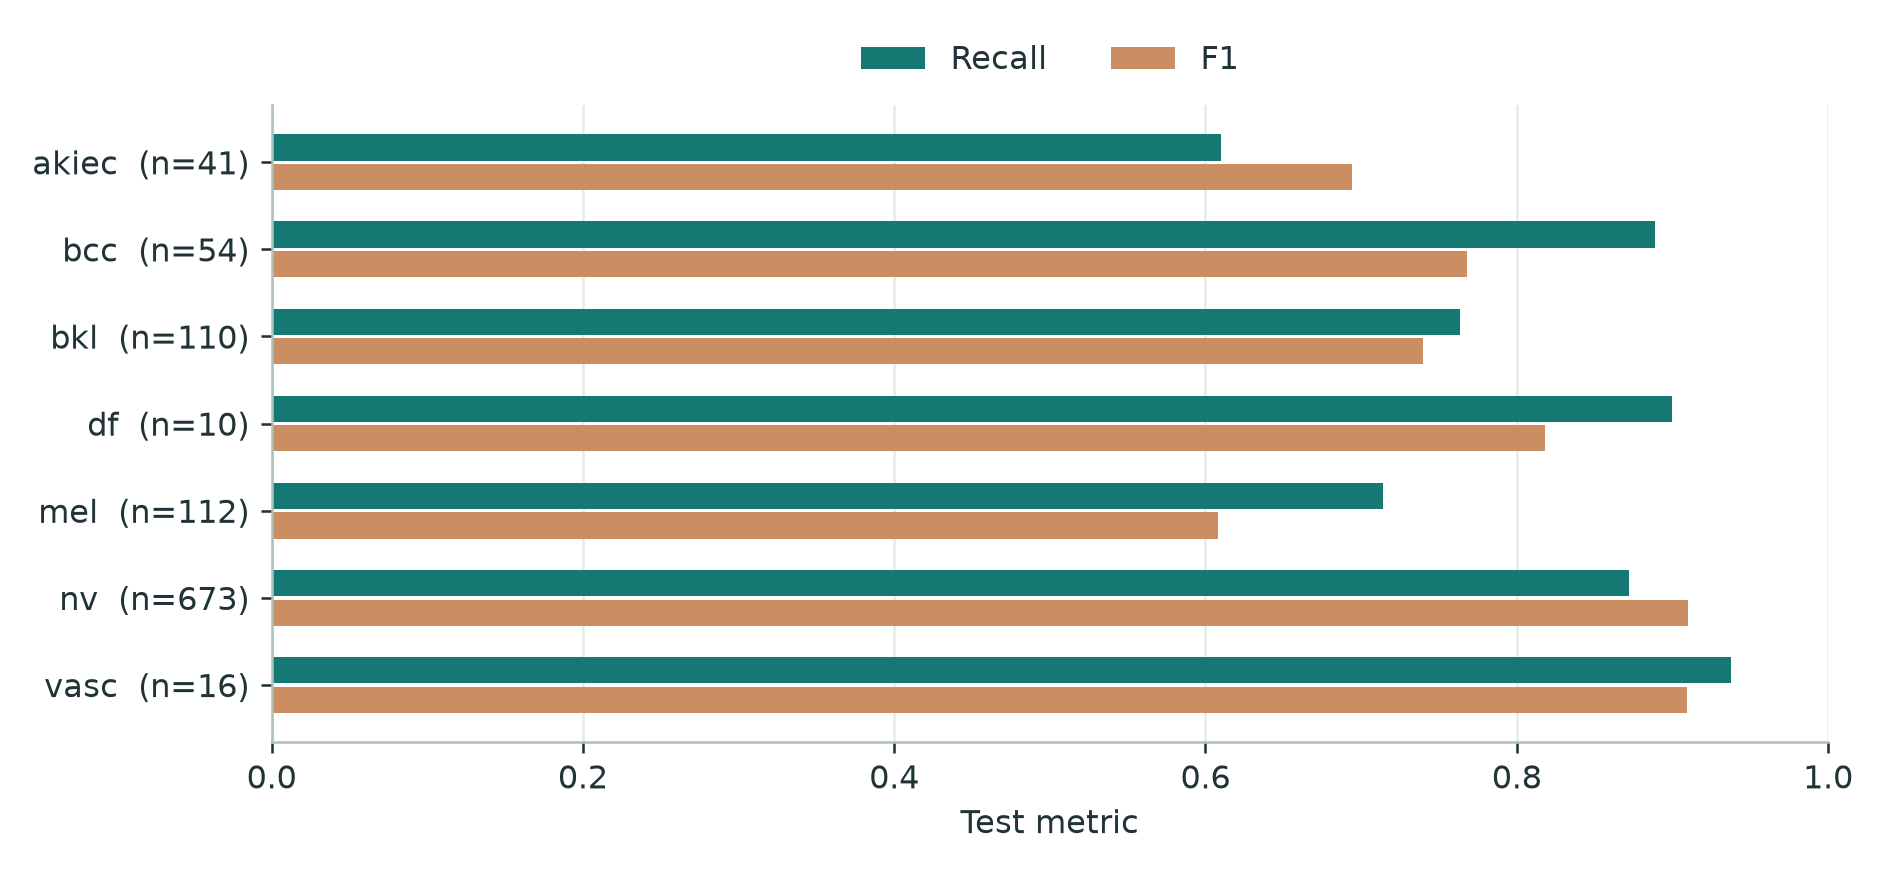
\includegraphics[width=\linewidth]{figures/per_class_recall_f1.png}
\end{minipage}\hfill
\begin{minipage}{.44\linewidth}
\centering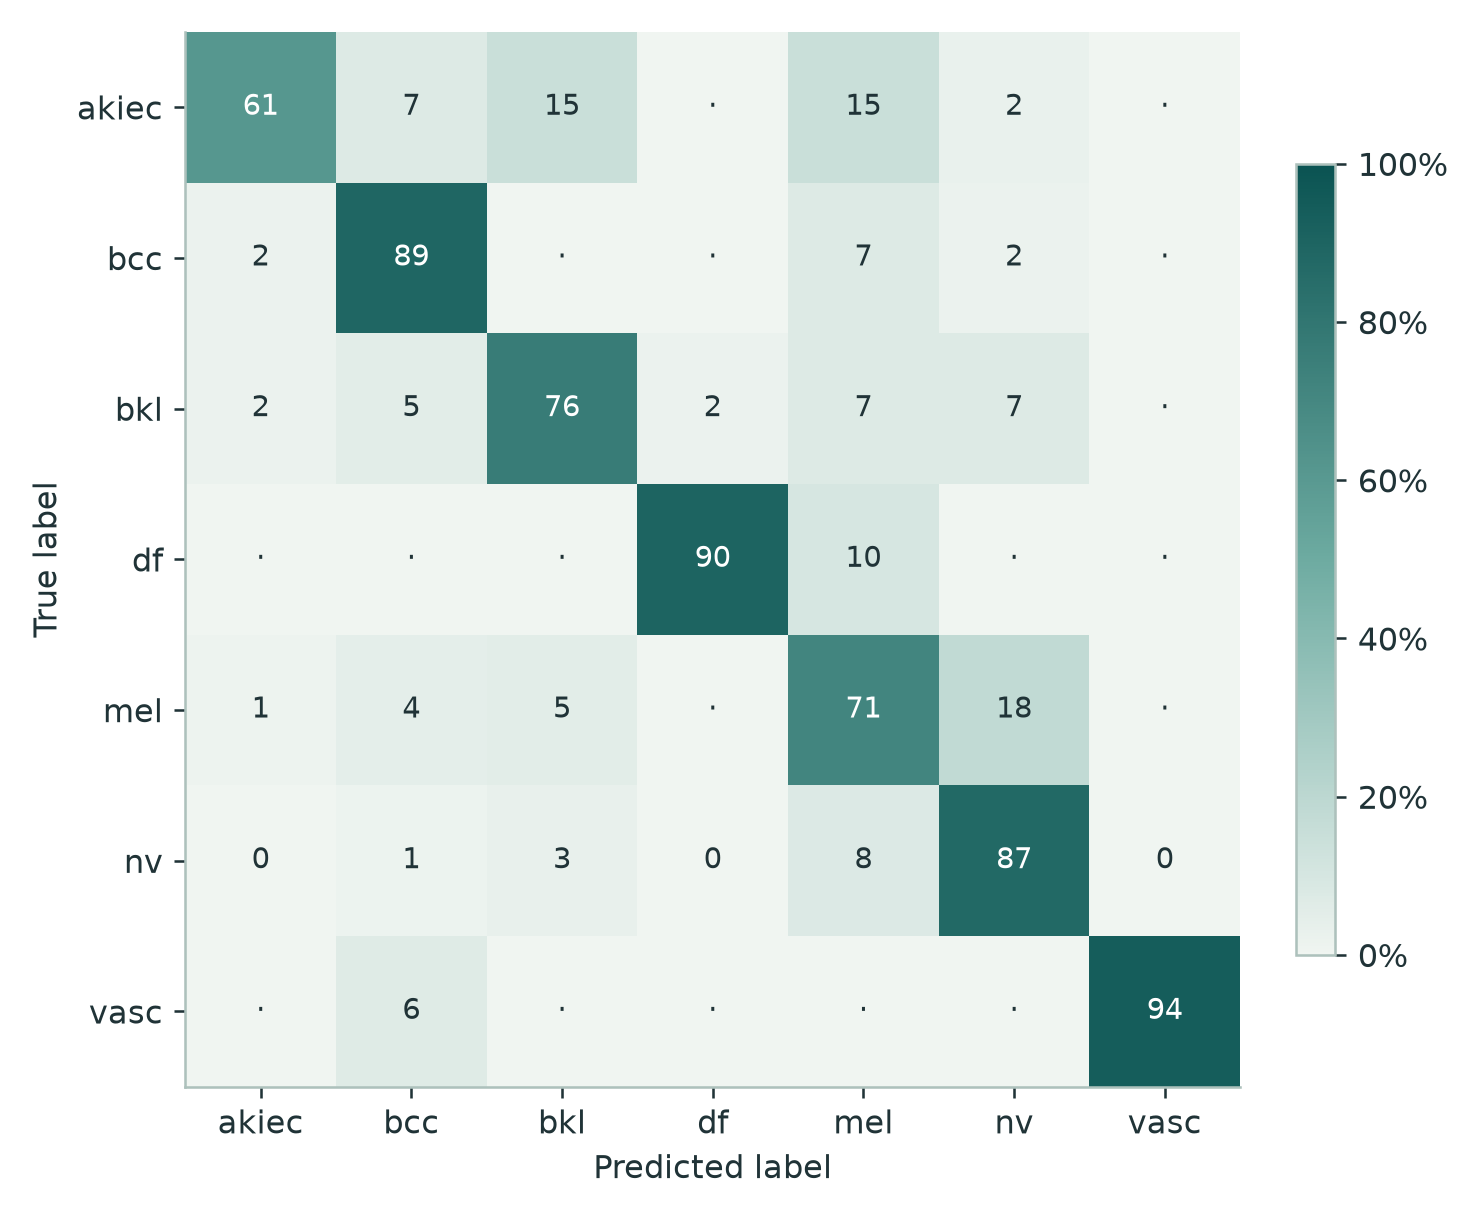
\includegraphics[width=\linewidth]{figures/normalized_confusion.png}
\end{minipage}
\captionof{figure}{Final-model recall and F1 (left) and row-normalized confusion matrix (right). Test support appears beside each class. The confusion-matrix diagonal gives recall.}
\label{fig:classresults}
\end{minipage}\par

\clearpage
\subsection{Calibration and Coverage}
We grouped the largest predicted class scores into ten equal-width bins. In each bin we compared the mean score with observed accuracy. The expected calibration error (ECE) \citep{guo2017} was the bin-size-weighted mean absolute difference, 0.0725 on the test set. A confidence score is not a reliable probability. The band above 0.9 was less accurate than the band below it, and 55 incorrect predictions had a score of at least 0.8.

\begin{minipage}{\linewidth}
\captionof{table}{Observed accuracy in the upper score bands.}
\label{tab:calibration}
\centering\small
\begin{tabular}{@{}lrrr@{}}
\toprule
Score interval & Images & Correct & Accuracy\\
\midrule
\([0.7,0.8)\) & 115 & 85 & 73.9\%\\
\([0.8,0.9)\) & 643 & 602 & 93.6\%\\
\([0.9,1.0]\) & 99 & 85 & 85.9\%\\
\bottomrule
\end{tabular}
\end{minipage}

The coverage curve varies the minimum score used to retain an image. At a cutoff of 0.8, the retained accuracy was 92.6\% at 73.0\% coverage. Increasing the cutoff to 0.9 left 9.7\% coverage and lowered retained accuracy to 85.9\%. These values describe the test sample and do not determine a suitable decision threshold.

\par\medskip
\begin{minipage}{\linewidth}
\centering
\begin{minipage}{.45\linewidth}
\centering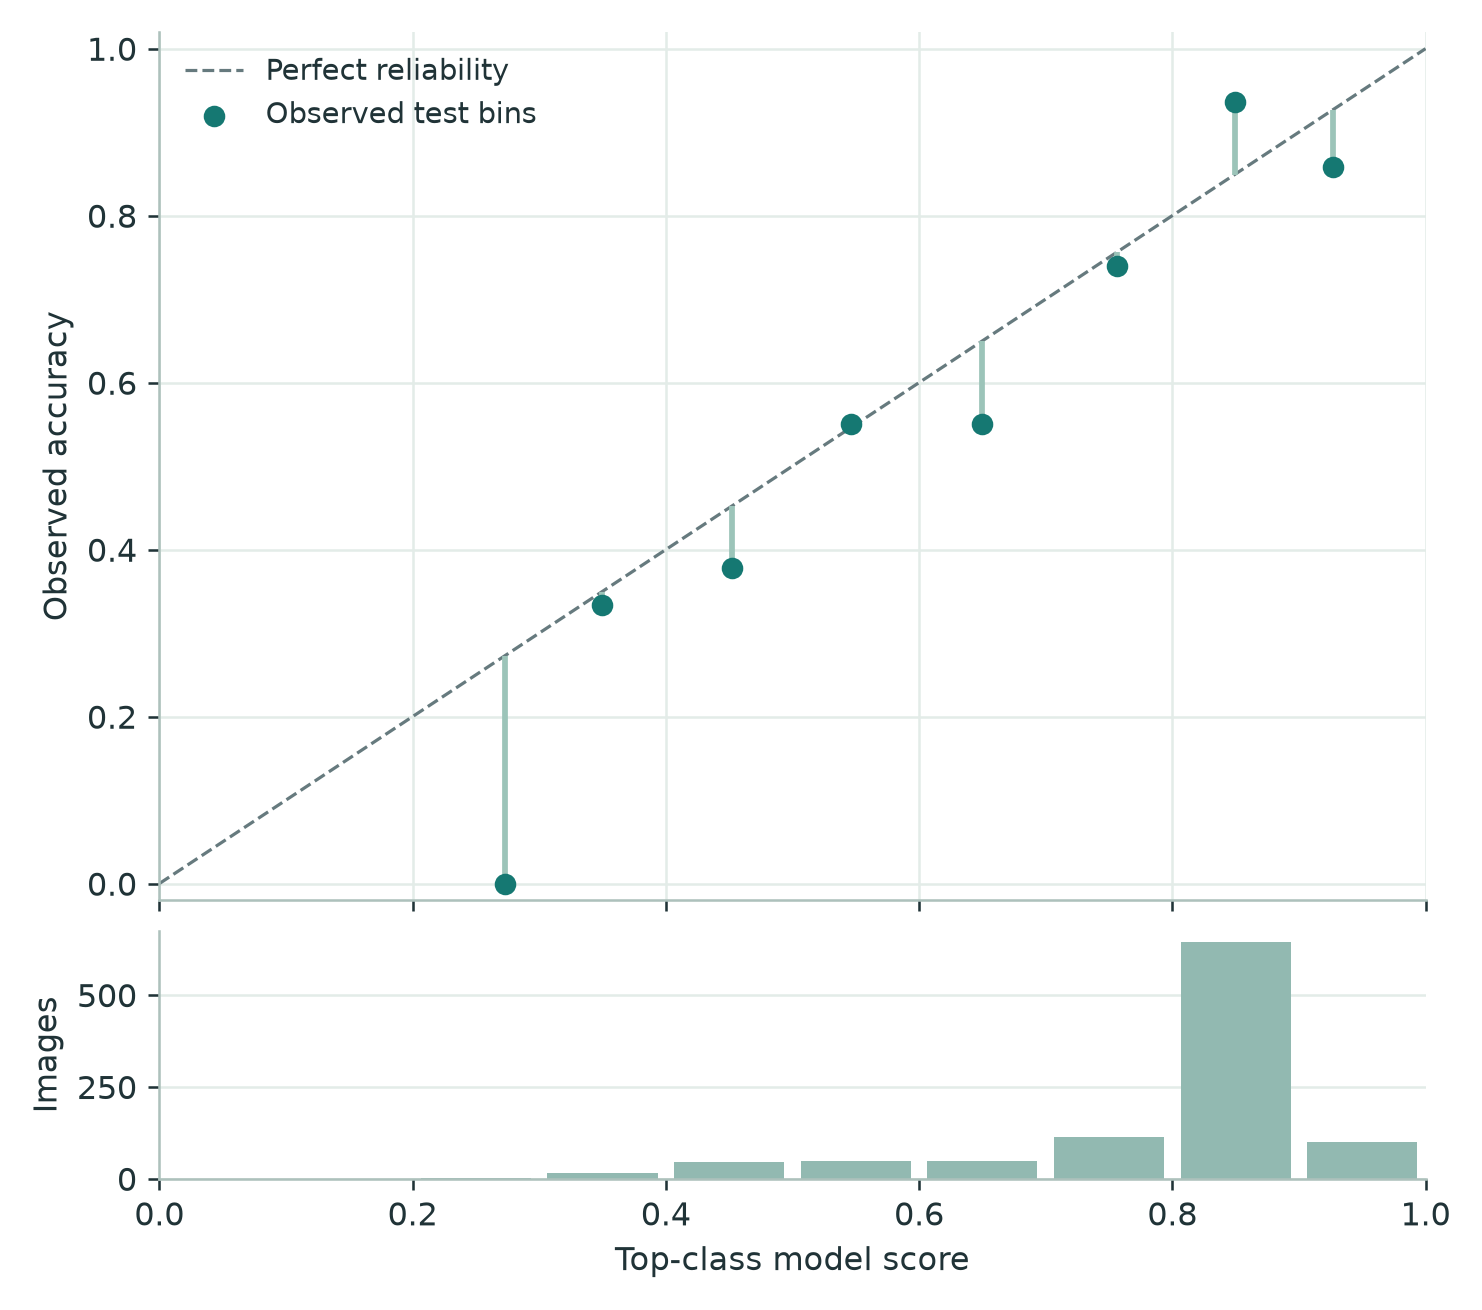
\includegraphics[width=\linewidth]{figures/reliability.png}
\end{minipage}\hfill
\begin{minipage}{.53\linewidth}
\centering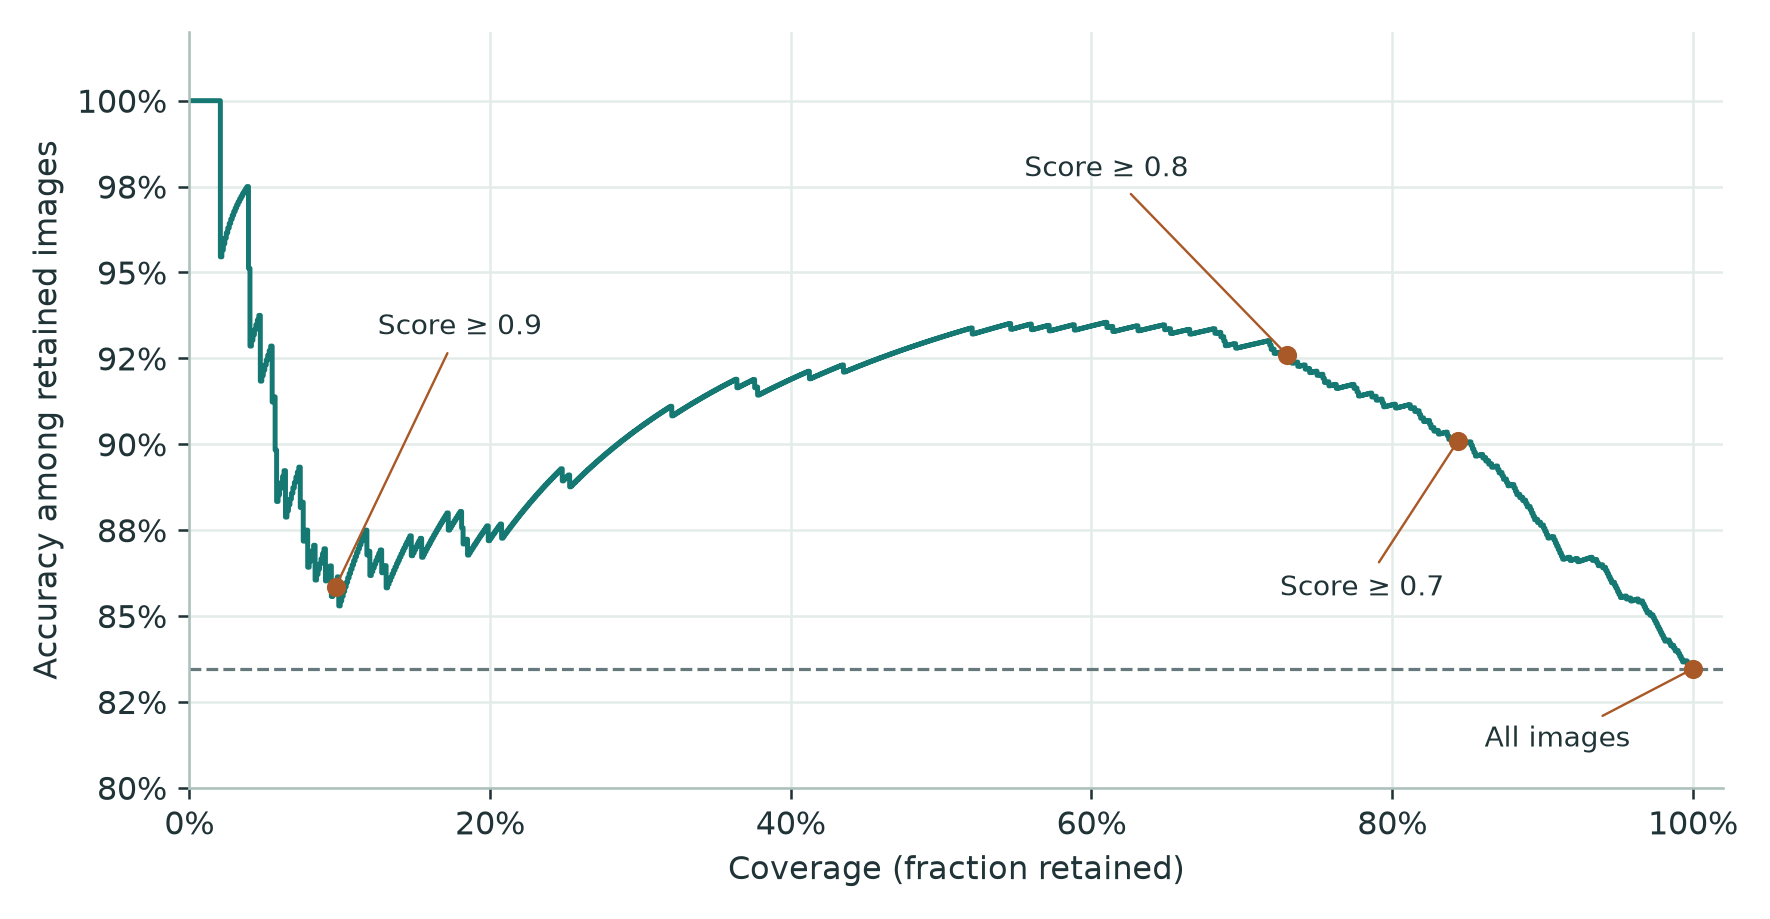
\includegraphics[width=\linewidth]{figures/coverage_accuracy.png}
\end{minipage}
\captionof{figure}{Reliability by score bin (left) and retained accuracy against coverage (right). The bar chart counts images per score bin. The coverage chart marks selected score cutoffs.}
\label{fig:calibration}
\end{minipage}\par

\subsection{Unsuccessful Variants}
Mixup and CutMix with a larger set of test-time transforms did not improve the selected ConvNeXt run's test macro-F1. Validation-fitted offsets also failed to carry their validation gain over to the hybrid test set. On the hybrid, the offsets raised validation macro-F1 from 0.7095 to 0.8030 and lowered the corresponding test score from 0.7691 to 0.7644. The metadata-fusion branch did not give us a better model than the image-only recipe. It also changed other settings, which prevents an isolated estimate of the effect of metadata.

\clearpage
\subsection{Grad-CAM}
We used gradients of the chosen class score to weight the final convolutional feature maps \citep{selvaraju2017}. We aligned the flipped views before combining the maps and overlaid the result on the image. In correctly classified cases, strong responses often overlapped the visible lesion. Similar overlap also appeared in wrong predictions, so a plausible-looking overlay does not establish correctness.

\par\medskip
\begin{minipage}{\linewidth}
\centering
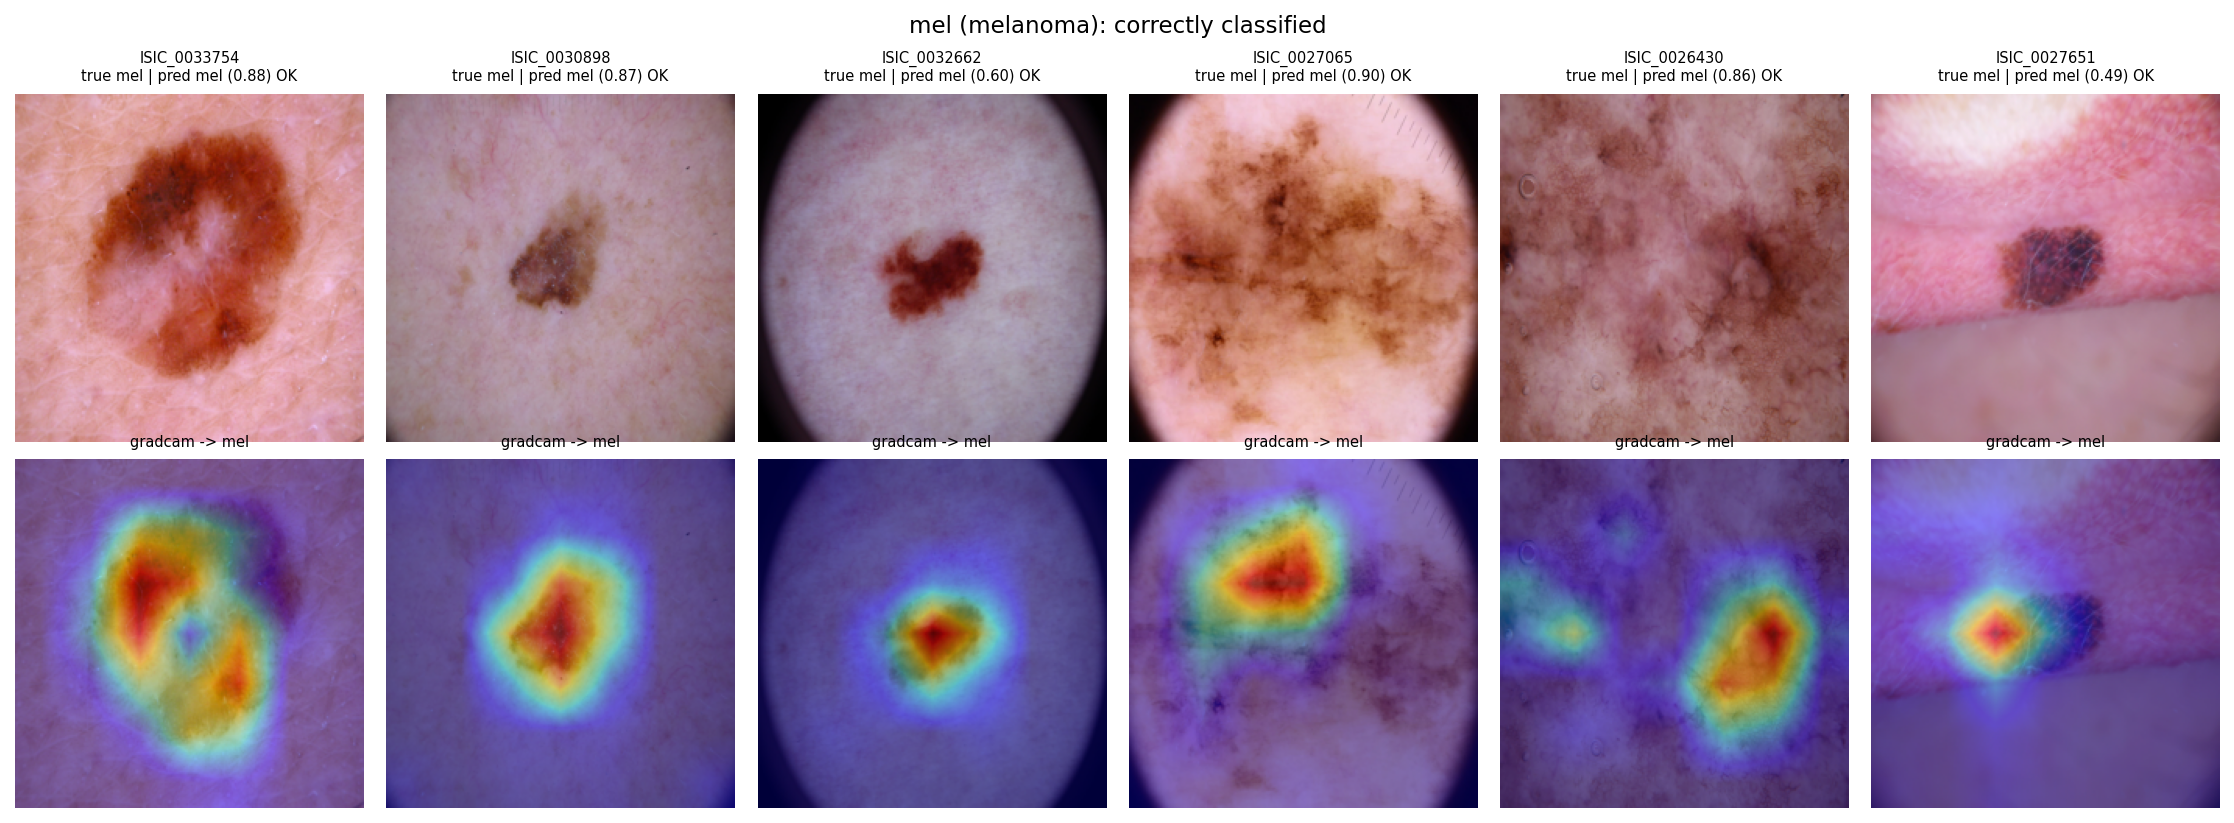
\includegraphics[width=.73\linewidth]{figures/gradcam_melanoma.png}\par\smallskip
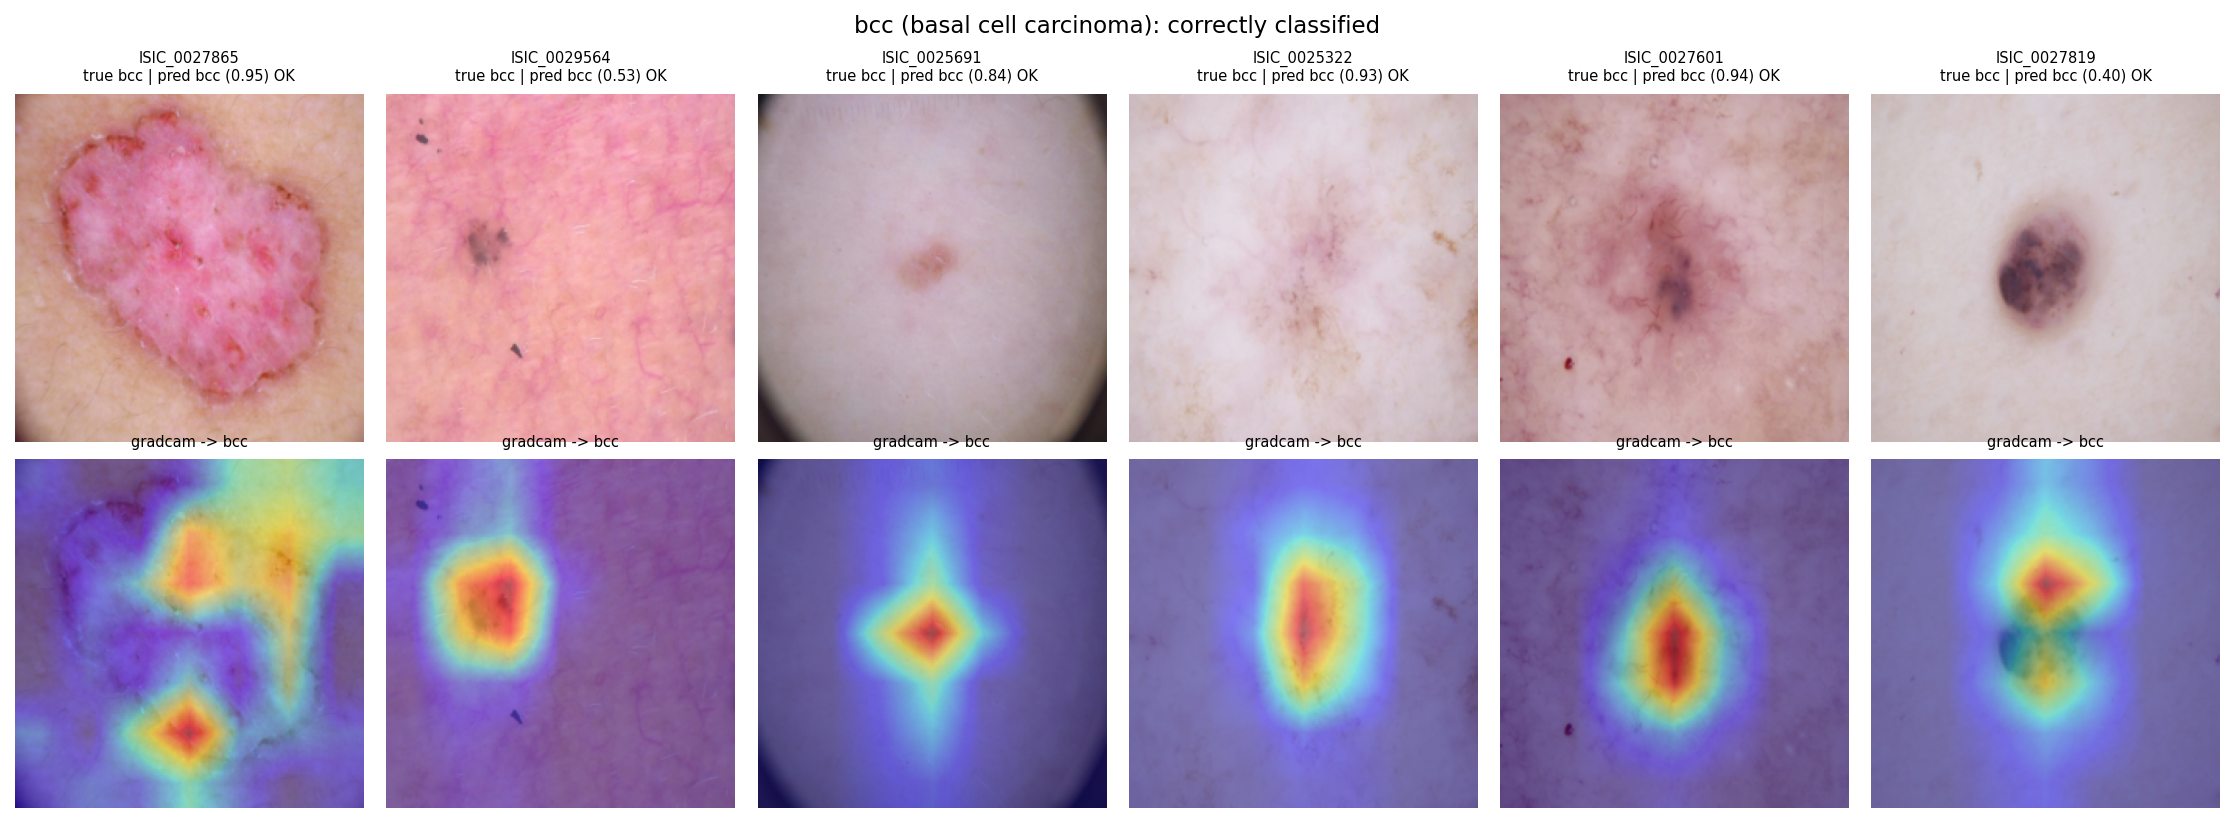
\includegraphics[width=.73\linewidth]{figures/gradcam_bcc.png}
\captionof{figure}{Original views and Grad-CAM overlays for correctly classified melanomas and basal cell carcinomas.}
\label{fig:gradcam-correct}
\end{minipage}\par
\reportfigure{.73}{gradcam_nevi_errors.png}{Grad-CAM for nevi assigned to the melanoma class. Some maps extend across the surrounding skin.}{fig:gradcam-errors}
\reportfigure{.79}{gradcam_method_comparison.png}{Grad-CAM and Grad-CAM++ on the same images \citep{chattopadhay2018}. Differences in intensity and extent reflect the explanation methods.}{fig:gradcam-compare}

\clearpage
\subsection{Error Gallery}
The galleries show two directions of error. Nevi classified as melanoma were the most frequent pair of wrong labels. The actinic keratosis and intraepithelial carcinoma group was much smaller, and six of its test images were assigned to benign keratosis-like lesions. The red labels call out wrong predictions with scores of at least 0.8. Scores displayed with a Grad-CAM panel can differ from the test-gallery score for the same image because the explanation pass recomputes the prediction.

\reportfigure{.94}{gallery_nevi_as_melanoma.png}{Examples of nevi classified as melanoma. The gallery shows the model scores for the predicted and true classes.}{fig:gallery-nv}
\reportfigure{.94}{gallery_akiec_as_bkl.png}{Actinic keratoses or intraepithelial carcinoma images classified as benign keratosis-like lesions.}{fig:gallery-akiec}

\clearpage
\subsection{Web Application}
The application is available at \href{https://skin-lesion-classification-umber.vercel.app/}{https://skin-lesion-classification-umber.vercel.app/}. The React interface accepts an image upload and sends it to a FastAPI backend for preprocessing and classification. The results view displays the predicted label, the top three candidates and their model scores. The user can request a Grad-CAM overlay and download a PDF summary. The web prediction uses a single image view. The evaluation results in this report used flip averaging. The application and its export state that they are intended for educational use and do not provide a diagnosis.

\par\medskip
\begin{minipage}[t]{.45\linewidth}
\vspace{0pt}\centering

\includegraphics[width=\linewidth,trim=0 880bp 0 0,clip]{figures/web_upload_mobile.jpg}
\captionof{figure}{Image upload screen.}
\label{fig:web-upload}
\end{minipage}\hfill
\begin{minipage}[t]{.53\linewidth}
\vspace{0pt}\centering
\screen{196mm}{web_about_mobile.jpg}
\captionof{figure}{Dataset overview, model design and held-out metrics shown in the application.}
\label{fig:web-about}
\end{minipage}

\clearpage
\begin{minipage}{\linewidth}
\centering
\begin{minipage}{.40\linewidth}
\centering\screen{124mm}{web_mobile_results.jpg}
\captionof{figure}{Mobile results with scores and a Grad-CAM overlay.}
\label{fig:web-results}
\end{minipage}\hfill
\begin{minipage}{.57\linewidth}
\centering\screen{124mm}{web_pdf_export.png}
\captionof{figure}{PDF export for a separate example.}
\label{fig:web-pdf}
\end{minipage}
\end{minipage}\par\medskip

\section{Conclusion}
\textbf{Findings.} ResNet-50 improved from 0.6542 to 0.7447 macro-F1 after changes to weighting, sampling and training-image deduplication. Stronger optimization and seed averaging brought the raw ensemble to 0.7815. Our final ConvNeXt-Tiny reached 0.7783 macro-F1 and 0.8123 balanced accuracy from a single checkpoint without fitted offsets. The detailed errors and calibration analysis show why performance should be reported by class and confidence band as well as in aggregate.

\textbf{Limitations.} The results come from one dermoscopic dataset and one held-out split. The smallest classes supply little evidence for stable rankings. Residual image similarity can survive lesion grouping, and the measurements are image-level. The results do not measure performance on new clinics or acquisition devices. Grad-CAM illustrates score sensitivity in selected examples, and the web application demonstrates the model in an educational setting.

\textbf{Future work.} We would repeat the comparison on additional lesion-grouped splits and an external cohort, with more examples of rare classes. Matching changes one at a time would help separate the effects of sampling, weighting and augmentation. A separate calibration set would allow confidence calibration and threshold selection to be evaluated without using the test images for either choice.

\clearpage
\begingroup
\urlstyle{same}
\providecommand{\doi}[1]{\href{https://doi.org/#1}{\nolinkurl{#1}}}
\renewcommand{\bibsection}{\section{References}}
\renewcommand{\bibfont}{\footnotesize}
\setlength{\bibsep}{0pt}
\bibliographystyle{unsrtnat}
\bibliography{references}
\endgroup

\par\begin{minipage}{\linewidth}
\section{Contributions}
Table~\ref{tab:contributions} lists each member's contribution, and the abstract and reference checks were shared. The complex-model column gives each member's reporting assignment.

\smallskip
\begin{minipage}{\linewidth}
\captionof{table}{Individual contributions.}
\label{tab:contributions}
\small
\renewcommand{\arraystretch}{1.12}
\begin{tabularx}{\linewidth}{@{}L{.157\linewidth}L{.171\linewidth}L{.156\linewidth}Y@{}}
\toprule
Member & Baseline built & Complex model analysis & Writing responsibility\\
\midrule
N. Deepak & Keras custom CNN & Swin-T & Introduction and Dataset\\
V. Sai Nikhil & Plain ResNet-50 & EfficientNet-B3 & Method and imbalance experiments\\
S. Sai Lohith & EfficientNet-B0 & EfficientNet-B3 + Swin-T & Survey and model comparison\\
D. Revanth Reddy & PyTorch CustomCNN & TransNet & Interpretation, web application and Conclusion\\
\bottomrule
\end{tabularx}
\end{minipage}
\end{minipage}
\end{document}

